\documentclass[11pt]{report}
\usepackage{fullpage}
%\usepackage{sourcesanspro, sourcecodepro}
\usepackage{minted}
\usepackage{graphicx}
\usepackage{awesomebox}
\usepackage{hyperref}
\usepackage{float} % stops images from moving around
\usepackage[a4paper, total={6in, 8in}, margin=0.75in]{geometry}
\usepackage{etoolbox}
\makeatletter
\patchcmd{\chapter}{\if@openright\cleardoublepage\else\clearpage\fi}{}{}{}
\RequirePackage[T1]{fontenc}
\RequirePackage[default,light,black]{roboto}

% DarkMode
\usepackage{xcolor}
\pagecolor[rgb]{0,0,0} %black
\color[rgb]{0.7,0.7,0.7} %grey

\hypersetup{
    colorlinks=true,
    linkcolor=cyan,
    citecolor=cyan,
    filecolor=cyan,
    urlcolor=cyan,
    pdfborder={0 0 0}
}

\graphicspath{{./images/}}

\title{APSC 258: Lab 3 Manual}
\author{Andre Cox \\ Scott Halston}

\begin{document}
\maketitle
\tableofcontents

\clearpage

\chapter{Introduction}
In the previous lab, you learned how to control the PiCar using the provided Python API. Within this lab, you will learn how to receive video from the PiCar Camera and display it. In addition, you will also learn how to process the video to make it easier for a neural network to understand. To do this we will use the Open Computer Vision (OpenCV) library. 
Your goal should be that by the end of this lab, you will have successfully received a video input from your PiCar and processed this video for your future neural network. Alongside this goal, it is also expected that you will gain an understanding of HSV colour space.

\chapter{Start of the Lab}
\section{Setup}
On your laptop you will need to install OpenCV you can do this with the following command:
\begin{minted}[fontfamily=courier, style=monokai, breaklines, frame=single,framesep=10pt]{shell}
    pip install opencv-python  
\end{minted}

We are using the OpenCV library in order to obtain the video from our PiCar.  To accomplish this we will write some code.

You will need to create a new Python file called imageprocessing.py. We will write the code in this file.
Try to follow along with the provided code snippets below to understand how this works. 

\begin{minted}[linenos, fontfamily=courier, style=monokai, bgcolor=black, breaklines]{python}
    # first we import OpenCV 
    import cv2 as cv 
\end{minted}

Next, we will use OpenCV to get video from the PiCar using the built-in VideoCapture class.
\begin{minted}[linenos, fontfamily=courier, style=monokai, bgcolor=black, breaklines]{python}
    # we create a variable called ip to store the ip address of the PiCar
    ip = "192.168.0.10"
    # we create a VideoCapture object and tell it to use the ip address of the PiCar
    # as well we use the %s format to insert the ip address into the string
    cap = cv.VideoCapture("http://%s:8080/?action=stream" % ip)
\end{minted}

Following, we will use a while loop to get and display the video. Without this while loop, the video would be displayed once and then stop. This while loop allows the video feed to be displayed continuously.

\begin{minted}[linenos, fontfamily=courier, style=monokai, bgcolor=black, breaklines]{python}
    # we create a while loop to get and display the video
    while True:
        # we get the next frame from the video stored in frame
        # ret is a boolean that tells us if the frame was successfully retrieved
        # ret is short for return
        ret, frame = cap.read()
        # we display the frame
        cv.imshow("PiCar Video", frame)
        # we use the waitKey function to wait for a key press
        # if the key is q then we break out of the loop
        if cv.waitKey(1) & 0xFF == ord('q'):
            break
\end{minted}

If you’ve managed to follow along up until this point, great! Hopefully, this has been relatively easy so far.
Your next step is to connect to the PiCar's WiFi and then run the imageprocessing.py file you just created to receive the video feed. If successful, you should see a window open with the PiCar's video streaming to it.

\chapter{Image Processing}
In the last chapter, we got the video from the PiCar Camera and displayed it. In this chapter, we will learn how to process the video to make it easier for a neural network to understand. To do this we will use the OpenCV library to isolate the green colour channel. We chose to isolate green because the painter's tape we are using to create our tracks is green. 

\pagebreak

\section{Theory}
The theory for why we are isolating green is very simple. We will use the HSV colour space to isolate the green colour. The HSV colour space is used to represent a colour in terms of Hue, Saturation, and Value. The Hue is the colour, the Saturation is the intensity of the colour, and the Value is the brightness of the colour. You may already be familiar with the RGB colour space where Red, Green, and Blue are mixed with each other to create any colour. We use the HSV colour space because it is much easier to isolate a range of colours. All we have to do is specify a range of Hue values.

\begin{figure}[htbp]
    \centering
    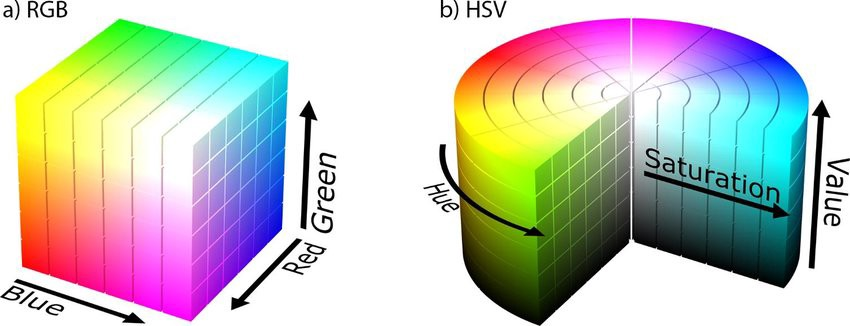
\includegraphics[width=0.8\textwidth]{HSVVSRGB.jpeg}
    \caption{HSV Color Space and RGB Color Space}
    \label{fig:HSVVSRGB}
\end{figure}

From the figure above we can see the RGB colour space is a bit confusing. How would we go about isolating the green colour? 
Isolating in the HSV colour space is much easier.

\section{Practice}
Let's practice isolating for green. To do this we will modify the code we wrote in the previous chapter. Let's add some code to make it find a range of green.

\begin{minted}[linenos, fontfamily=courier, style=monokai, bgcolor=black, breaklines]{python}
    # we create a while loop to get and display the video
    while True:
        # we get the next frame from the video stored in frame
        # ret is a boolean that tells us if the frame was successfully retrieved
        # ret is short for return
        ret, frame = cap.read()
        # we display the frame
        cv.imshow("PiCar Video", frame)

        # now we convert the frame to the HSV color space
        hsv = cv.cvtColor(frame, cv.COLOR_BGR2HSV)

        # I found that these ranges work well for green
        # However you can change the ranges to find other colors
        mask = cv.inRange(hsv, (40, 50, 90), (100, 255, 220))

        # now we display the mask
        cv.imshow("Mask", mask)

        # we use the waitKey function to wait for a key press
        # if the key is q then we break out of the loop
        if cv.waitKey(1) & 0xFF == ord('q'):
            break

\end{minted}

When you run the modified code you should see two windows open. The first window is the PiCar's video and the second window is the mask. The mask is a binary image that is white where the green is and black where there is no green. Remember you need to be connected to the PiCar's WiFi to see the PiCar's video.

\notebox{
    \textbf{Reasons for Image Processing:}
    Image processing is used when there is a lot of data that could confuse a neural network. Through image processing, we can get rid of the data that is not needed. In our situation, we just removed approximately 2/3 of our data; which means, our neural network will learn much faster
}

\chapter{End of the Lab}
Now we have a processed video stream that can be used to train a neural network. In the next lab, we will train a simple neural network to recognize our track.



\end{document}